\subsection{Hardware Details}

\subsubsection{Housing}
%from bottom to top

Here the design of the housing shown in fig.~\ref{fig:CALISMechanism} is described in more detail. Starting at the gate valve inside the clean room CRH on which CALIS has been installed, a a teflon disk allows to electrically isolate CALIS from ground, even though during normal operations the CALIS housing is also connected to ground. A tripod with a bellow has been used to vertically align the housing right after installation on the gate valve. The bellow is connected to a 23.375" long cylindrical stainless steel enclosure pipe. It has the same diameter as the organ pipe (6'') and leads into a view port (depicted in blue in fig.~\ref{fig:CALISMechanism}) and which is the access point for accessing the source arm and exchanging sources.  

Above the view port is the upper assembly, which is a stainless steel cylindrical enclosure that houses the cable drive mechanism, including the cable spools the stepper motor and the articulation mechanism, already described in Sec.~\ref{sec:DeploymentArticulation}. 

CALIS offers various safety features to ensure that the device runs smoothly, no components are lost inside the detector, avoid any contamination of the detector by dirty or incompatible materials, maintain pressure and avoid introduction of oxygen or water in contact with the LS and TMB, operation in the volume that excludes possibility of contact with PMTs or light pulsers (pacman) attached to each PMT.
 
\subsubsection{Safety features}

\begin{description}

\item[Drive mechanism:]
The drive mechanism is a stepper motor that has an integrated absolute encoder providing the location of the source at all times, even in the event of a power failure. In the event of a power failure, the magnetic break ensures there is no movement of the pig. The torque of the servo motor is limited in case of an unexpected load. 

The speed reducer (gears) is a double worm gear design. The primary worm gear has a 50:1 reduction and the secondary worm has a 82:1 reduction. The input speed of the servo motor is 2400 RPMs and the output is 0.6 RPM and has the weight capacity of 148 lbs. In the event of a power failure the speed reducer has the ability to hold the load at any position without back drive. The speed of the motor has been limited to 0.4\,cm/s which minimizes any lateral oscillation of the pig during lowering and raising the source. Additionally, this is the maximum speed at which the motor is not overheating.

\item[Manual retraction system:]
In the unlikely case of a complete motor failure while the source is deployed, it is possible to manually retract the pig back to its home position and close the gate valve. The motor is disengaged, and wrench is used to manually wind the cable back onthe spools and retract the pig back above the gate valve. 

\item[Cable strength and length:]
The cables holding the pig have been rated for loads over 590\,kg, while the weight of the pig is at the level of 10-15\,kg so well below the breaking strength of the cable. The cable length has been established so that the maximum depth at which the pig can be deployed is above the level of the PMTs inside the LSV. In case, the command is given to deploy to greater depth, the cable completely unwinds and then rewinds in the opposite direction, which then effectively retracts the pig to a higher z-position until the preset motor count of steps is reached. 

%% is this true?

   
\item[Upper limit switch:]
The motor has an absolute encoder and step position is never lost even in the case when the motor loses power. When the pig has reached its home position within the upper assembly it will stop.  However, if the top of the pig continues past its home position (based on the number of steps given), it will not be able to pass its home position thanks to the upper limit switch that will be triggered in that case. 

Neither the manual retraction system has been used nor has the upper limit switch been activated during calibration campaigns.


     
\item[Light and leak tightness of CALIS:]
When the deployment device is next to the cryostat the gate valve is open and we take also data with the LSV. A prerequisite is that the housing is absolute light tight and pressure leak tight. All view ports have light tight covers for when the organ pipe gate valve is open. Both light and leak tightness has been extensively validated throughout the manufacturing process until including commissioning (Sec.~\ref{sec:Commissioning}).

\end{description}
	
%%%%%%%%%%%%%%%%%%%%%%%%%%%%%%%%%%%%%%%%%
%%%%%%%%%%%%%%%%%%%%%%%%%%%%%%%%%%%%%%%%%

\subsubsection{Deployment device}
The pig (Fig. \ref{fig:sourcePod_arrows}) contains the support structure for the arm which holds the source at its end.  This piece is equipped with tapered cones on the top and bottom that ensure that the ends do not get snagged on inner edges of the organ pipe as it is moving up and down. It is attached to the housing by two cables.  Swivel hooks are employed in the attachment of the cables to the pig that allow the cables to move freely and not get tangled. 
There are two weights built into the device, one cylindrical in the conical cap above the rotation gear mechanism and one inside the cones at the bottom end of the device. Both help to minimize any lateral motion or oscillations during deployment and articulation and dearticulation especially. It also ensures smooth motion of the deployment device into the organ pipe and back to the home position inside the housing.

\subsubsection{Source holder and arms}
A source arm and the source holder are attached to the articulation gear (Fig.~\ref{fig:SourceHolder}). Different arm lengths have been prepared with a maximum arm length of 62 cm, the arm length thereby being measured from the pivot point of the rotation gear to the tip of the source holder. This arm length allows the source to be placed in immediate contact with the cryostat (Fig.~\ref{fig:CALIS_photos}, right), as the center axis of the organ pipe is 81 cm from the TPC center and the cryostat has an outer radius of 32 cm. The 62 cm arm was used for most of the deployments in the past calibration campaigns (Sec.~\ref{sec:CalibCampaign}). Inside the source holder the radioactive source is placed, pressed to the tip and held in place via a spring during deployment, articulation and dearticulation. The source holder is sealed such that no liquid scintillator can enter during the deployment. This has also been verified during each source extraction, that no liquid was found on the inside.

\begin{figure}[htbp]
 \centering
  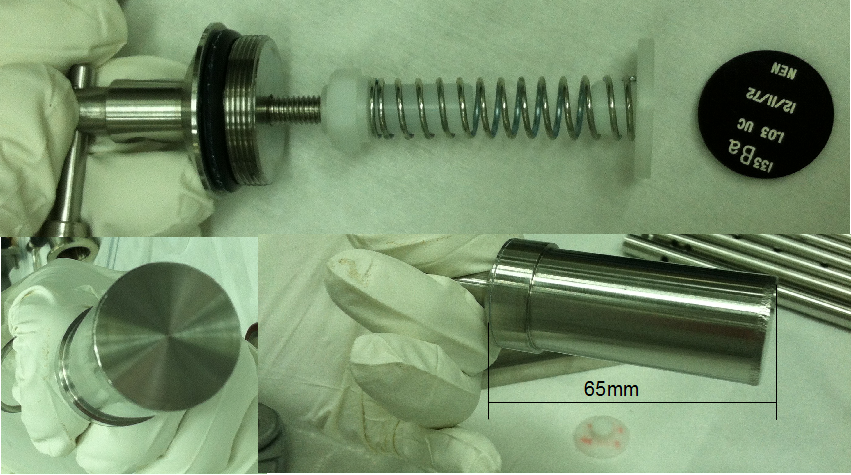
\includegraphics[width=0.7\textwidth]{Figures/SourceHolder.png}
  \caption{Source holder that connects to an arm and to the articulation gear of the deployment device. The source, here a $^{133}$Ba source is pressed to the tip of the source holder via a spring.}
  \label{fig:SourceHolder}
\end{figure}


\subsubsection{Securing of the source}
All connection points for the source and arm have been secured with two push locking pins that cannot be disengaged without a person pressing the pin. 
The source holder is held in place via a locking mechanism and two locking pins. When the source is attached to the arm, the source container must be slid over a protruding pin. There is a sliding locking mechanism that interlocks onto the pin. Once the source is locked into position there are 2 additional locking pins that are put into place (one above and one below the source holder pin), each of which have a button that must be depressed in order for the pins to be released. In addition, the source holder and the 2 locking pins will all be tethered from outside the view port until they are locked in place eliminating the possibility of accidental falling.  The tethering will happen before installation of the source and before the removal of the source. The cables used to tether the pins and the source holder during installation and removal will be detached after installation and prior to deployment to avoid the possibility of the arm getting entangled.  
 
%\begin{figure}[htbp]
 %\centering
% 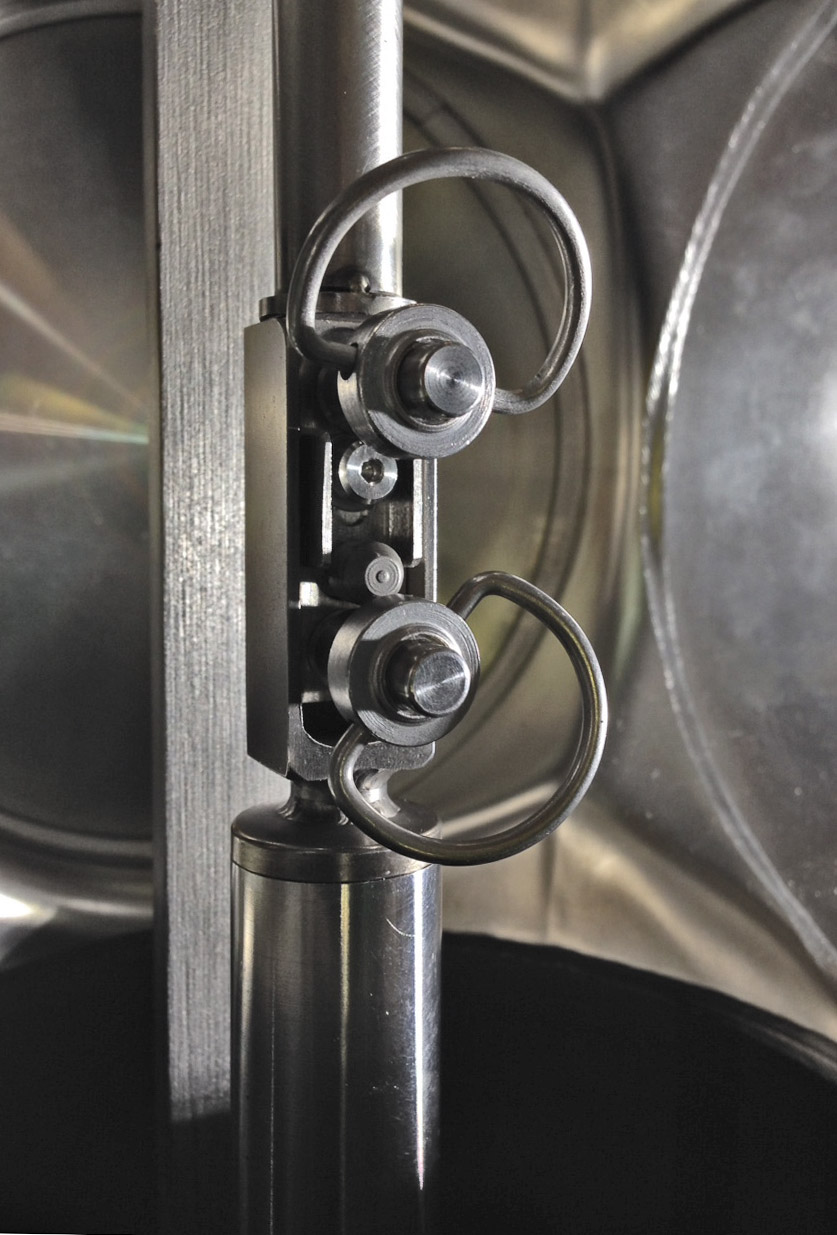
\includegraphics[width=3.2in]{Figures/sourceHolder_locking}
% \caption{Locking mechanism for the source holder. This photo shows two push pins that ensure that the sliding pin stays in place and the the source holder %cannot under any circumstances get detached from the arm.  The only way to remove the push pins is to depress buttons on each of them by hand. }
% \label{fig:sourceHolder_locking}
%\end{figure}

%\begin{figure}[htbp]
% \centering
 % \includegraphics[width=7in]{Figures/sourceAttachmentParts}
%  \caption{Components of the source attachment mechanism. Central image shows how the pin that holds the source holder slides down and prevents the %source from getting loose.  The slide pin is locked in place by two push pins shown in Fig. \ref{fig:sourceHolder_locking}}
%  \label{fig:sourceAttachmentParts}
%\end{figure}
